\section{PX4 SITL simulation and validation}
\label{sec:test-2-sitl}

Section \ref{sec:devenv} describes the software-in-the-loop simulation mode developed by PX4.
This mode will enable testing and validating the correct operation of individual components of the program's architecture in several distinct steps before integrating them into one control flow.
These initial tests will ensure that the foundational features of the control algorithms, sending commands to the autopilot and retrieving images for analysis, are dependable.
To do that, the following steps will be checked in order:
\begin{enumerate}
    \item Verify that it is possible to start the simulated flight controller and that it connects to the 3D simulator.
    \item Connect the DroneVisionControl program to the flight controller and send basic commands.
    \item Retrieve images from a camera and feed them to the computer vision detection utility.
\end{enumerate}

To reduce the amount of configuration needed for the first test, the Gazebo\footnote{\url{https://gazebosim.org/home}} simulator will be used instead of AirSim, since it is already installed during PX4's SITL setup.
Gazebo works natively on Linux, so it can run in parallel with the simulated flight stack and the developed application on the same WSL \acrshort{os}.
To set up the Linux system, PX4 and DroneVisionControl are installed as detailed in Appendix \ref{app:install-dev-env}.

Once both parts are installed, the simulation can be started with the \texttt{make\ px4\_sitl\ gazebo} command or using the \texttt{simulator.sh} script found on the project repository\footnote{\url{https://github.com/l-gonz/tfg-giaa-dronecontrol/blob/main/simulator.sh}}.
The result can be seen in Figure \ref{fig:gazebo}, with the user interface and 3D world of the Gazebo simulator on the left side and the PX4 console on the right side.
The console can be used to send commands to the vehicle and set configuration parameters for the simulation.

\begin{figure}[H]
  \centering
  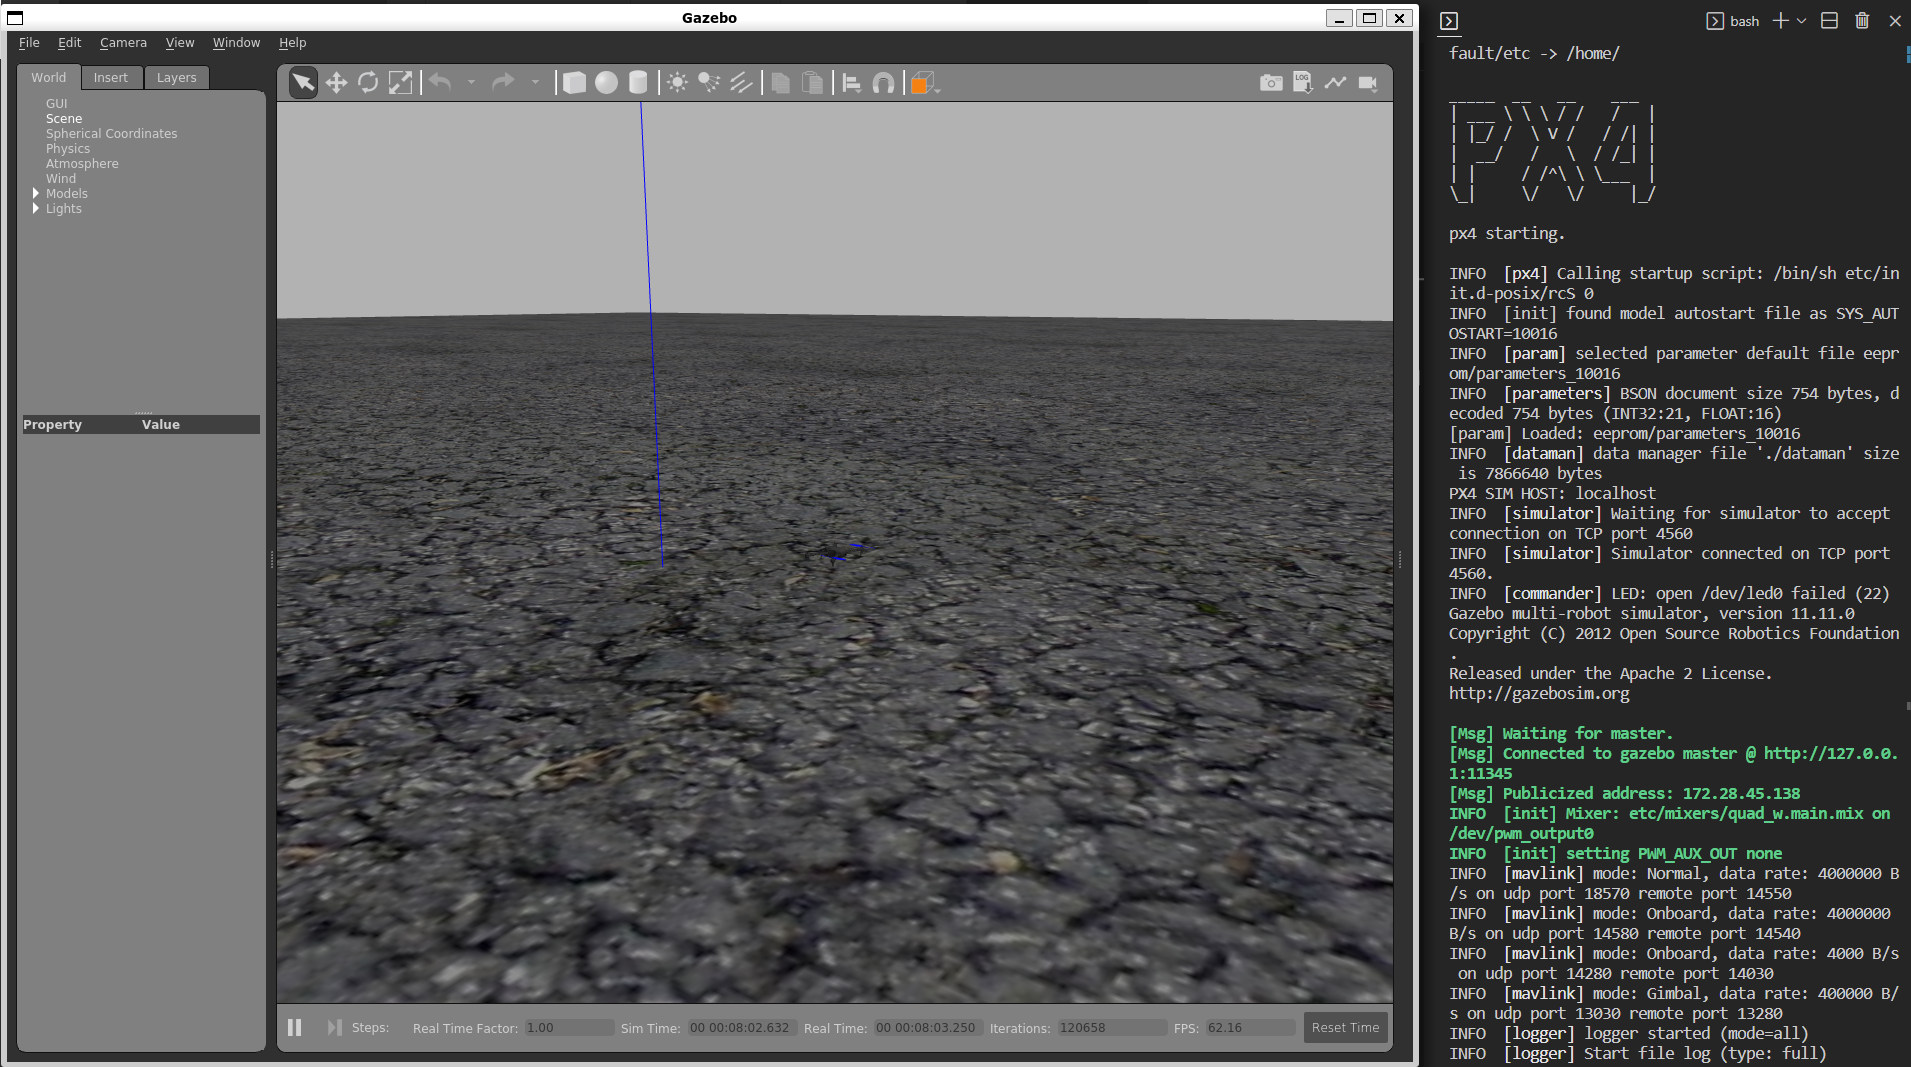
\includegraphics[width=\textwidth, keepaspectratio]{img/gazebo.png}
  \caption{Gazebo simulator (left) and output from the PX4 console (right) after PX4's software-in-the-loop simulation is started.}
  \label{fig:gazebo}
\end{figure}

The first command to test is takeoff, which is done by sending \texttt{commander takeoff} through the PX4 console.
Figure \ref{fig:gazebo-takeoff} shows the simulator's state after the takeoff command, where the vehicle model has climbed to the default takeoff height of 2.5 meters above the ground.
The command to land the vehicle again is \texttt{commander land}.

\begin{figure}
  \centering
  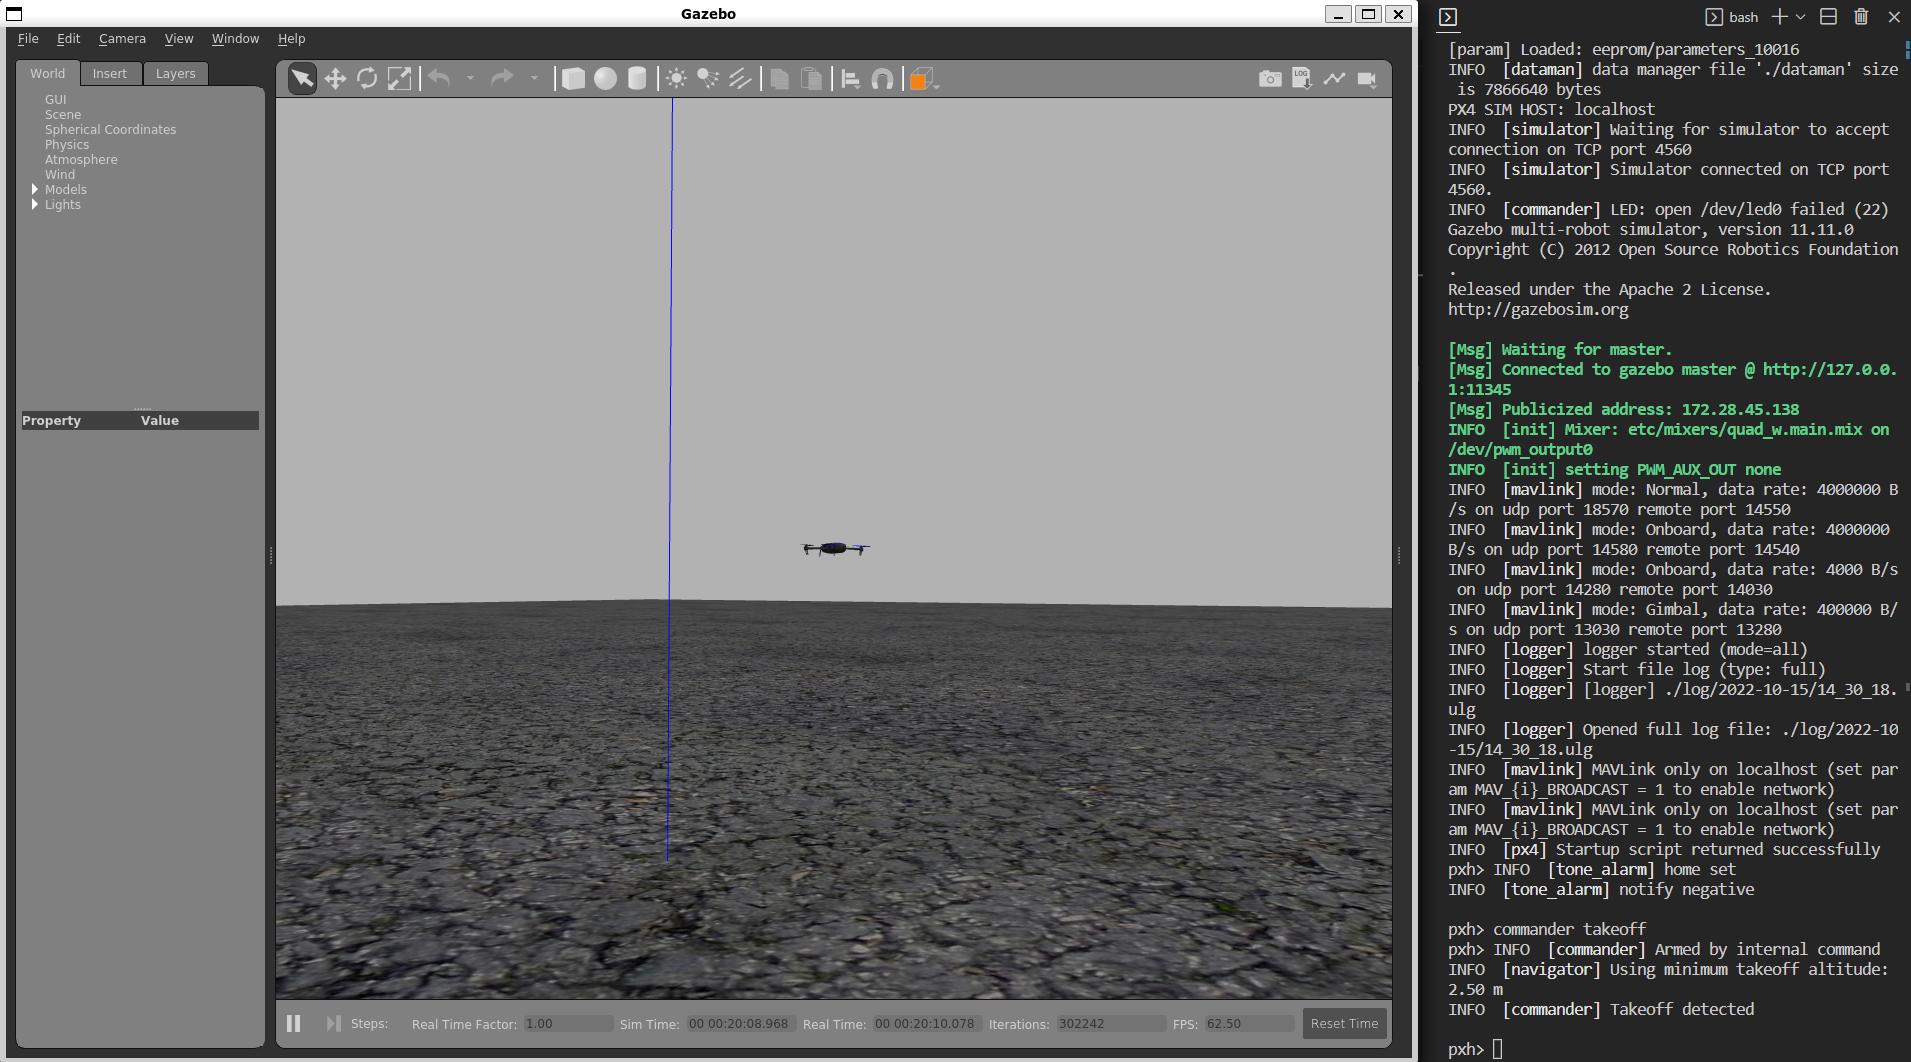
\includegraphics[width=\textwidth, keepaspectratio]{img/gazebo-takeoff.png}
  \caption{Gazebo simulator (left) and output from the PX4 terminal (right) after the takeoff command has been executed.}
  \label{fig:gazebo-takeoff}
\end{figure}


The second step is to connect the DroneVisionControl application to the simulation.
The \texttt{test-camera} utility described in Section \ref{subsec:cam-tool} has been developed specifically to test establishing a connection to PX4 SITL and process images without engaging any of the program's control modules.
It can be started through the tools section of the application's command-line interface (\texttt{dronevisioncontrol tools test-camera}).
Once the connection to the simulation is established successfully, movement commands can be sent to the vehicle through keyboard input.
For example, pressing the "T" key will trigger takeoff.
The result should be the same as sending the \texttt{commander takeoff} command through the PX4 console, verifying that the MAVSDK library and the pilot module work as expected.



For the last step of this test, a camera will be added to the system to retrieve images that can be sent onward to the computer vision algorithm.
The configuration used in the previous steps, however, needs some modifications, as WSL cannot access hardware devices or USB ports on the host computer.
The simplest solution is to migrate the DroneVisionControl application to the Windows system.
Since that is the environment chosen for the HITL tests that will be carried out later, it is also beneficial to validate at this point that the application can run without issues on Windows.
Appendix \ref{app:install-dev-env} contains the details on configuring the PX4 flight stack simulation to allow connecting to a MAVLink server through a different machine in the local network.
Once the application is installed in the Windows system, the same \texttt{test-camera} utility can be run with the \texttt{-c} option to retrieve images from a connected camera.
Additionally, the \texttt{-h} and \texttt{-p} options can be used to run the hand-detection and pose-detection algorithms, respectively, on the captured images.

Figure \ref{fig:sitl-hand} shows the image and text output of the program when the \texttt{test-camera} tool is run with the hand-detection feature activated.
On the left side, the detection algorithm tracks the shape of a hand detected in the image and on the right side, the logged information shows the connection being established and keyboard commands being sent to the simulator.

\begin{figure}
  \centering
  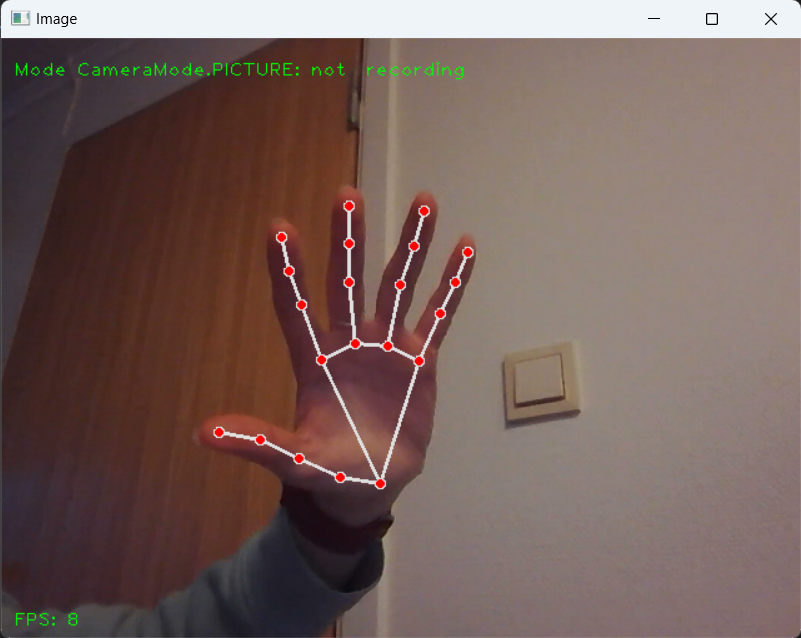
\includegraphics[width=\textwidth, keepaspectratio]{img/sitl-hand.png}
  \caption{Hand detection algorithm running on images taken from the computer's integrated webcam.}\label{fig:sitl-hand}
\end{figure}

After testing the flight stack, the default simulator and the developed application with its image retrieval, it is time to add the AirSim simulator to the environment.



\subsection{PX4 SITL validation with AirSim}
\label{sec:test-3-airsim}

The end goal for the development environment is to use the AirSim simulator to take advantage of its 3D-rendering and computer vision capabilities.
For this reason, it becomes necessary to validate that the new simulator can run correctly on Unreal Engine, interacting with PX4 as the default Gazebo simulator did. Additionally, all the necessary features for detection, tracking and following should work as expected.
These characteristics will be validated in the order below:
\begin{enumerate}
    \item Verify that the AirSim simulator can start, connect to the PX4 SITL through the WSL virtual network and receive commands from the PX4 terminal.
    \item Integrate the previous tests with AirSim by running the hand-gesture control solution described in Section \ref{sec:hands}.
    \item Check that the DroneVisionControl program can obtain images from the virtual camera inside AirSim's simulated world.
    \item Test the pose recognition algorithms on the images obtained from the AirSim simulation.
    \item Check that the follow solution can control the vehicle's velocity directly in PX4's offboard mode.
\end{enumerate}

In the first place, the AirSim simulator needs to be installed in the Windows host.
The complete installation process is described in appendix \ref{app:install-airsim}.
There are specific configuration parameters that have to be set to be able to connect the AirSim simulator in Windows to the PX4 SITL simulation running inside WSL.
On the simulator side, AirSim's settings file has to include a line defining the IP address of the network interface to use.
This parameter, along with the entire configuration file used for SITL testing, can be found in appendix \ref{app:airsim-config}.
On the PX4 side, it is necessary to specify that the simulator will attach through a different IP address than \texttt{localhost}.
This is done by setting the \texttt{PX4\_SIM\_HOST\_ADDR} environment variable in the Linux system to the IP address of the Windows host on the WSL virtual network before starting PX4 as follows:
\begin{minted}{bash}
export PX4_SIM_HOST_ADDR=[IP-address]
make px4_sitl none_iris
\end{minted}
These commands start the software-in-the-loop execution, which attempts to attach to an already running simulator listening on the IP address specified and the TCP port 4560, in this case, AirSim.
Therefore, every time either PX4 or AirSim stops its execution, both of them have to be stopped and the AirSim simulator restarted first.
Figure \ref{fig:airsim-sitl} shows the testing environment after the AirSim simulator and the PX4 console have been started successfully.
At this point, it is possible to use the PX4 console to send takeoff and land commands to the simulator and observe the 3D model of the vehicle climb into the air.

\begin{figure}
  \centering
  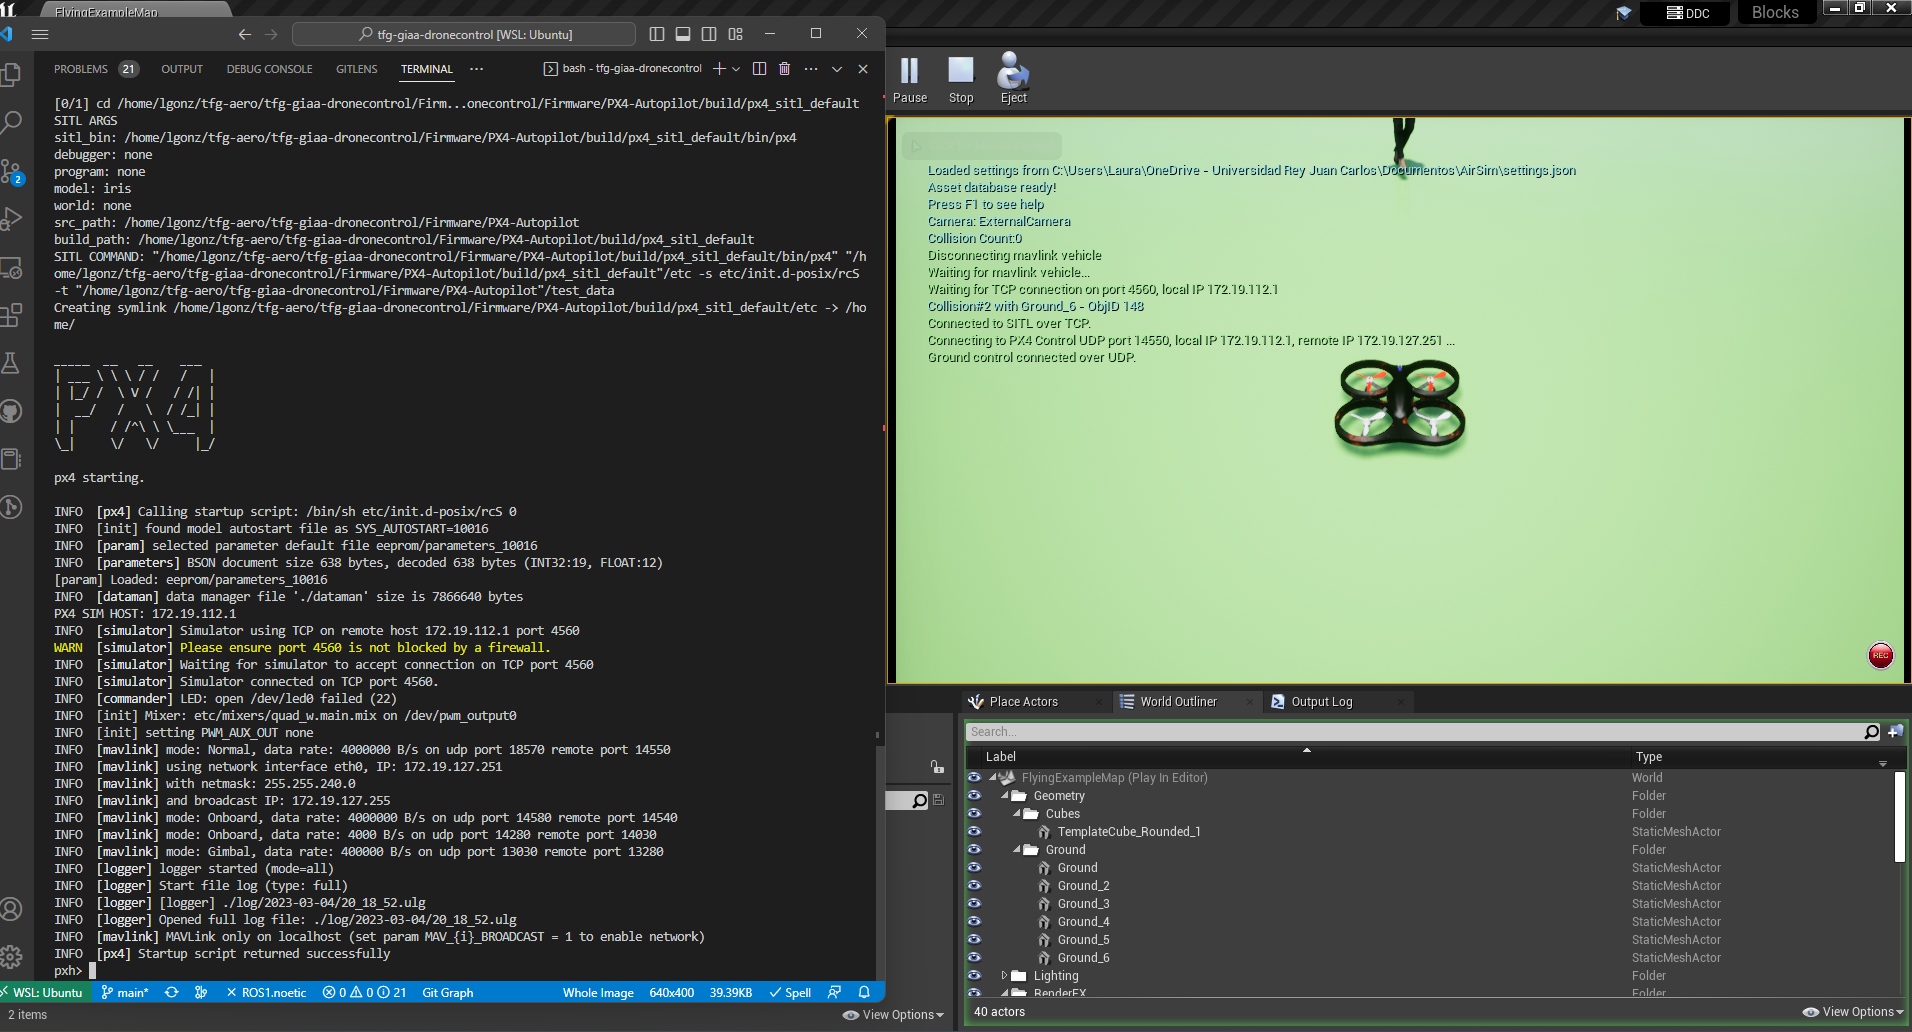
\includegraphics[width=\textwidth, keepaspectratio]{img/airsim-sitl.png}
  \caption{AirSim environment connected to PX4 flight stack running in SITL mode.}
  \label{fig:airsim-sitl}
\end{figure}

%%%%  FROM HERE GOOD WRITING


In the second test, all the previously validated individual components will be integrated with the AirSim simulator by executing the proof-of-concept control solution. Specifically, the DroneVisionControl application will run with the gesture-based control loop enabled. This test will be conducted on the Windows system to be able to rely on images from the physical camera.
The complete execution is shown in the video\footnote{\url{https://l-gonz.github.io/tfg-giaa-dronecontrol/videos/test-sitl-hand}} accessible through this \href{https://l-gonz.github.io/tfg-giaa-dronecontrol/videos/test-sitl-hand}{link}. Additionally, a frame extracted from the video can be observed in Figure \ref{fig:sitl-hand-video}.

\begin{figure}
  \centering
  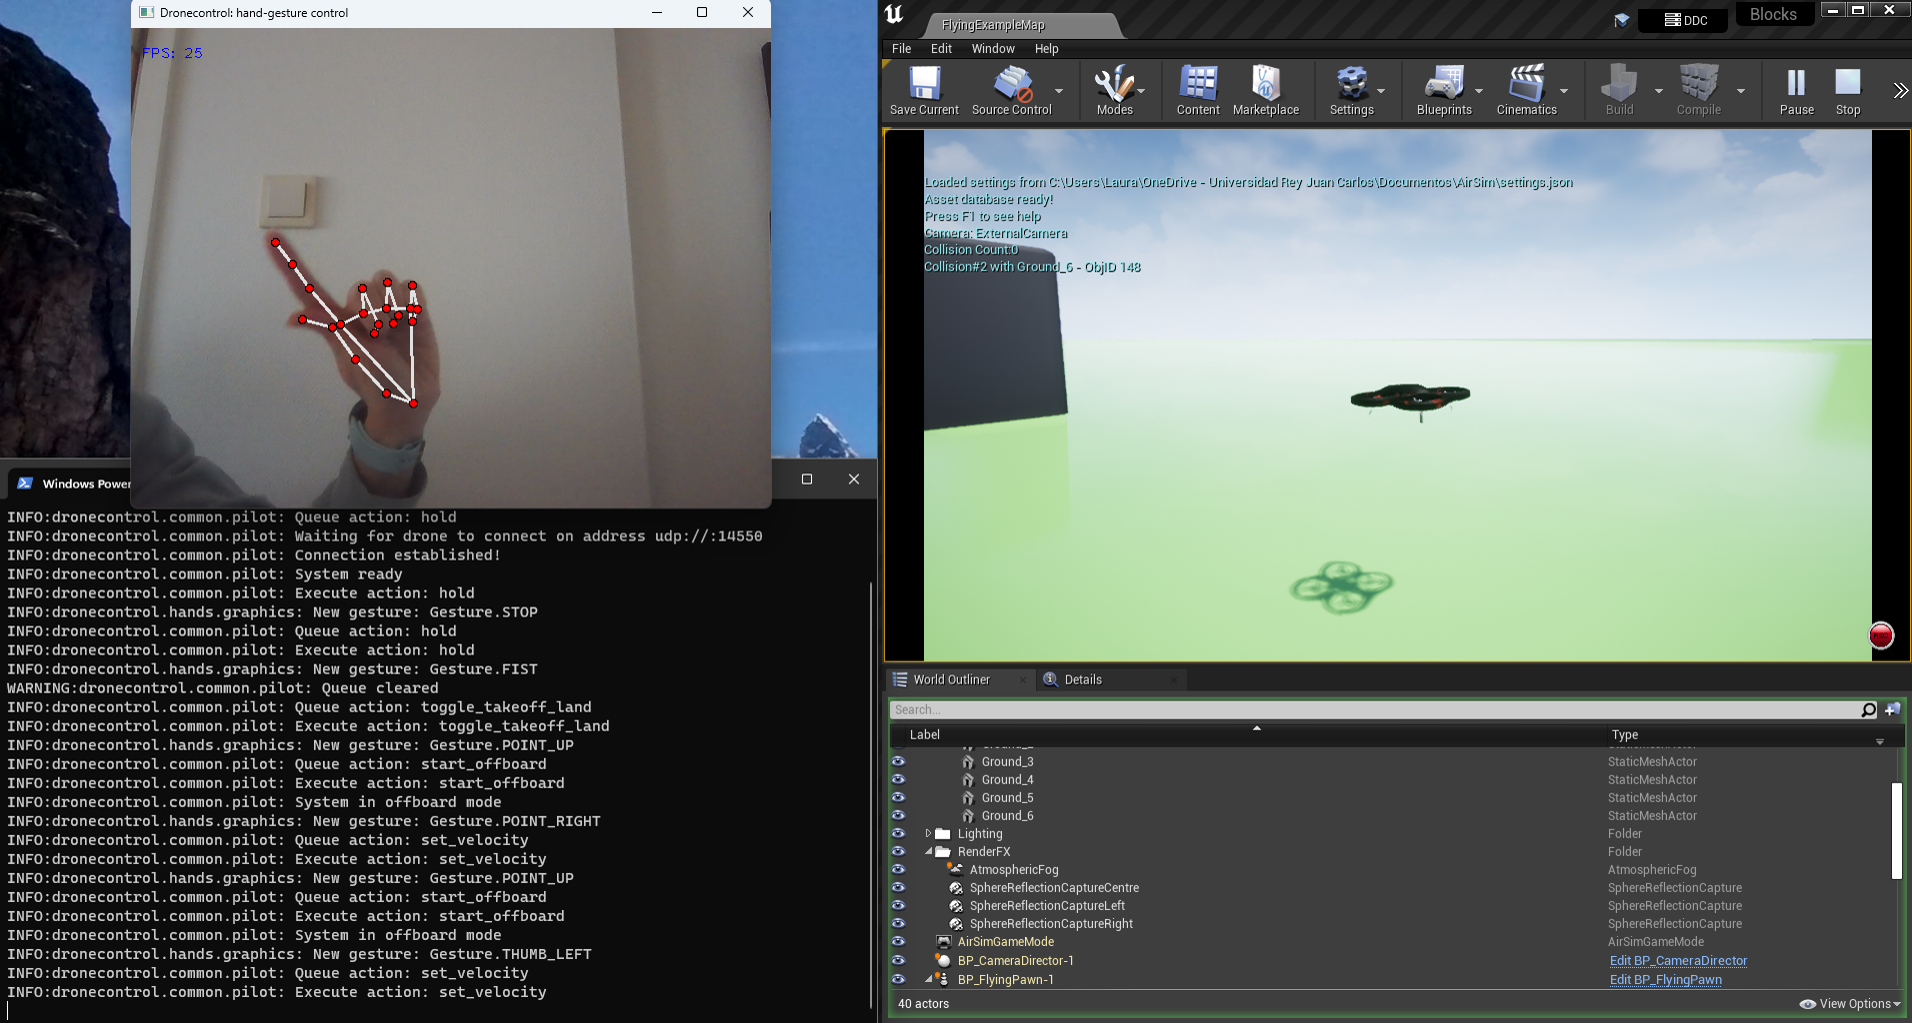
\includegraphics[width=\textwidth, keepaspectratio]{img/video-hand-sitl.png}
  \caption{Single frame extracted from the video of the full execution of the hand-gesture control solution. Gesture detection is shown on the upper left side of the screen. The lower left side shows the mapping between detected gestures and commands, and the right side shows the vehicle's movement response inside the simulator.}
  \label{fig:sitl-hand-video}
\end{figure}



The validation process will now shift its focus towards the tools required to execute the pose detection and tracking mechanism. To assess the detection and tracking of human figures from images captured within the simulator, the camera testing tool provided with DroneVisionControl can be employed once again.

Figure \ref{fig:airsim-sitl-pose} demonstrates the output obtained when running the tool with a 3D model of a person positioned in front of the drone within the simulated environment. The following command was executed: 
% \texttt{dronevisioncontrol tools test-camera -{}-wsl -{}-sim -{}-pose-detection}
\begin{minted}{bash}
dronevisioncontrol tools test-camera --wsl --sim --pose-detection
\end{minted}


In the image, the computer vision utility successfully detects the key features of the human body, outlining them with a bounding box. Simultaneously, the program's logged output displays two calculated positions in the terminal: the x-coordinate of the midpoint within the bounding box and the percentage of the image height covered by the height of the bounding box.
These two values serve as inputs for the PID controllers that drive the follow solution, as described in Section \ref{sec:follow}. The logs can be employed to calibrate the distance at which the drone is to track the person when the control mode is engaged. This is done by setting the simulated vehicle at the target distance from the person model and using the output height percentage as the set point for the forward PID controller.

\begin{figure}[H]
  \centering
  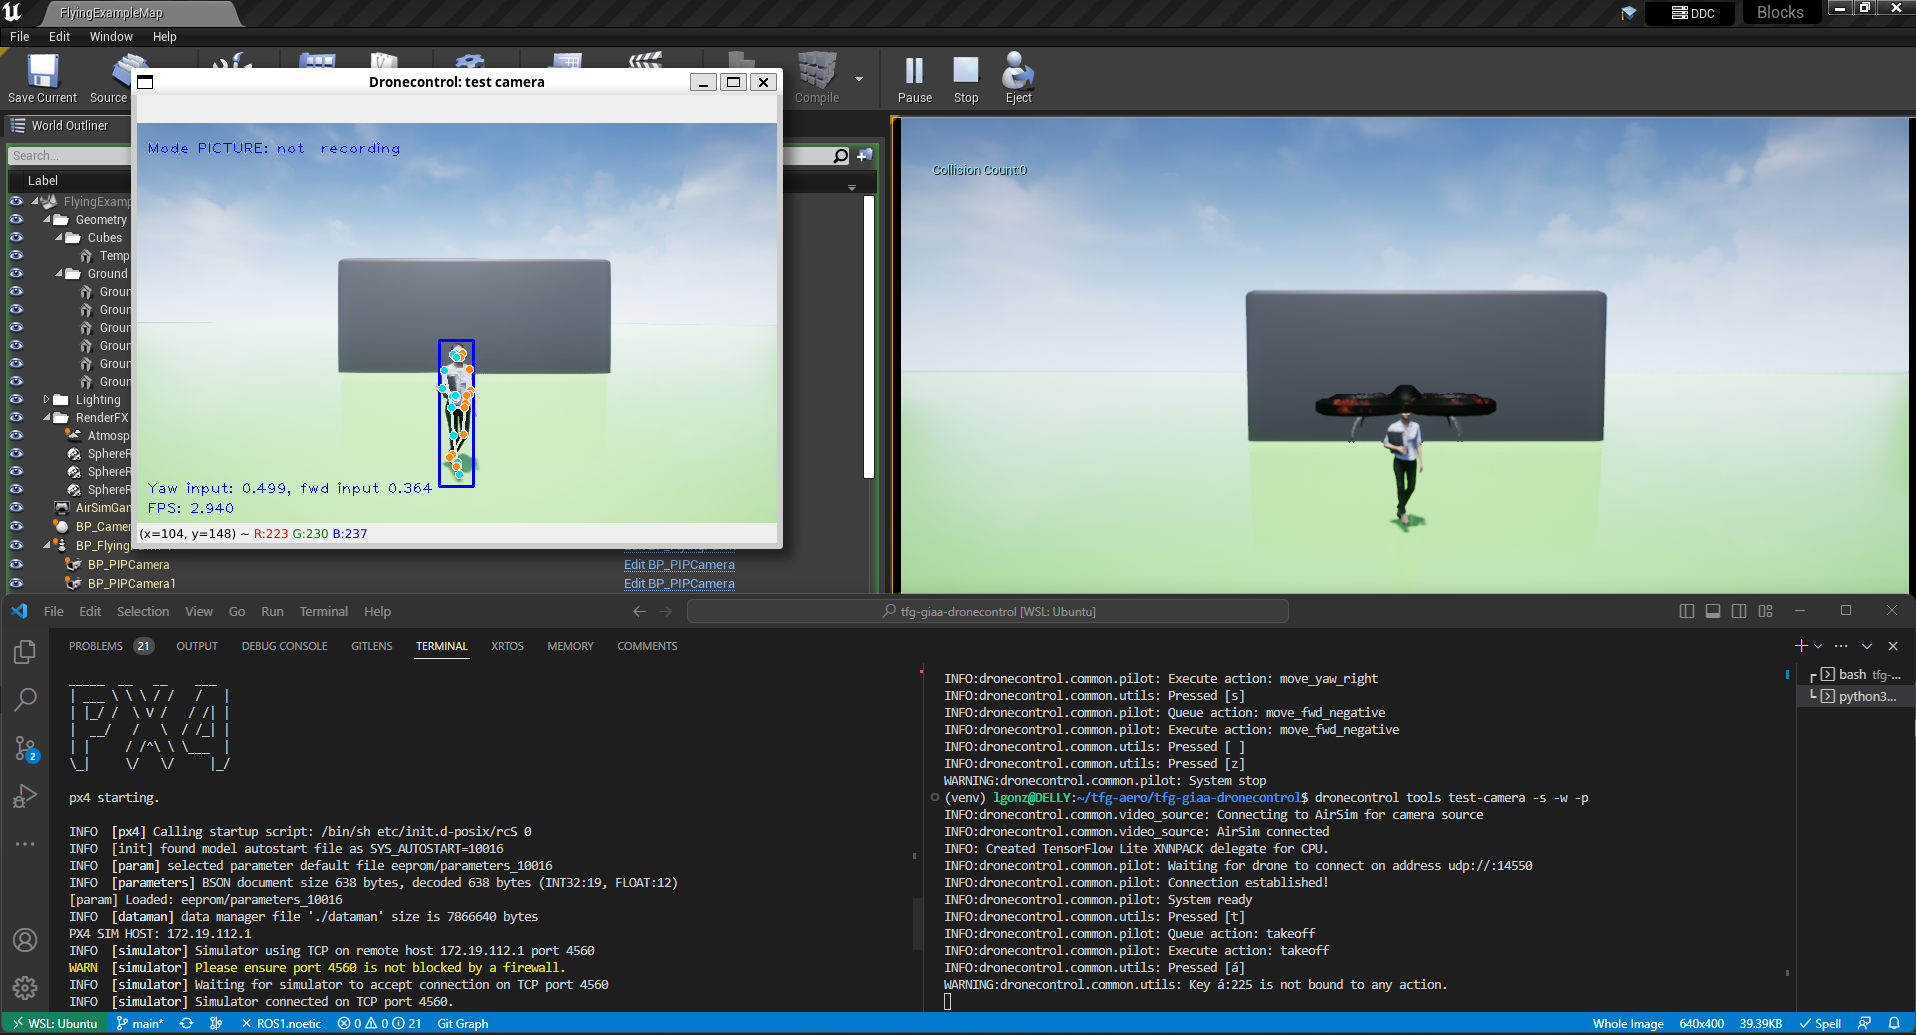
\includegraphics[width=\textwidth, keepaspectratio]{img/airsim-sitl-pose.png}
  \caption{AirSim, PX4 and DroneVisionControl applications running side-by-side and connecting to each other}
  \label{fig:airsim-sitl-pose}
\end{figure}

Before using the testing environment to fine-tune the PID controllers in the follow solution based on the vehicle's response, it is essential to confirm that the controllers can appropriately react to changes in the figure's position. This can be achieved by enabling only the proportional term of the controllers with a suitably low magnitude, ensuring slow and smooth movement. The expected result is that the vehicle starts moving forward when the person moves backwards and that it starts turning to the right when the person moves to the right, mirroring the movement in the remaining directions.

To run the follow control program with specific values for the proportional terms of the yaw and forward controllers (10 and 2, respectively), the following command can be used:

\begin{minted}{bash}
dronevisioncontrol follow --sim --yaw-pid (10, 0, 0) --fwd-pid (2, 0, 0)
\end{minted}